
\section{Introduzione} % Sections are added in order to organize your presentation into discrete blocks, all sections and subsections are automatically output to the table of contents as an overview of the talk but NOT output in the presentation as separate slides

%------------------------------------------------

\begin{frame}
\frametitle{Transformer}
\textbf{Self-attention-based architectures}, in particular Transformers, have become the model of choice in natural language processing.
\vspace{0.5cm}

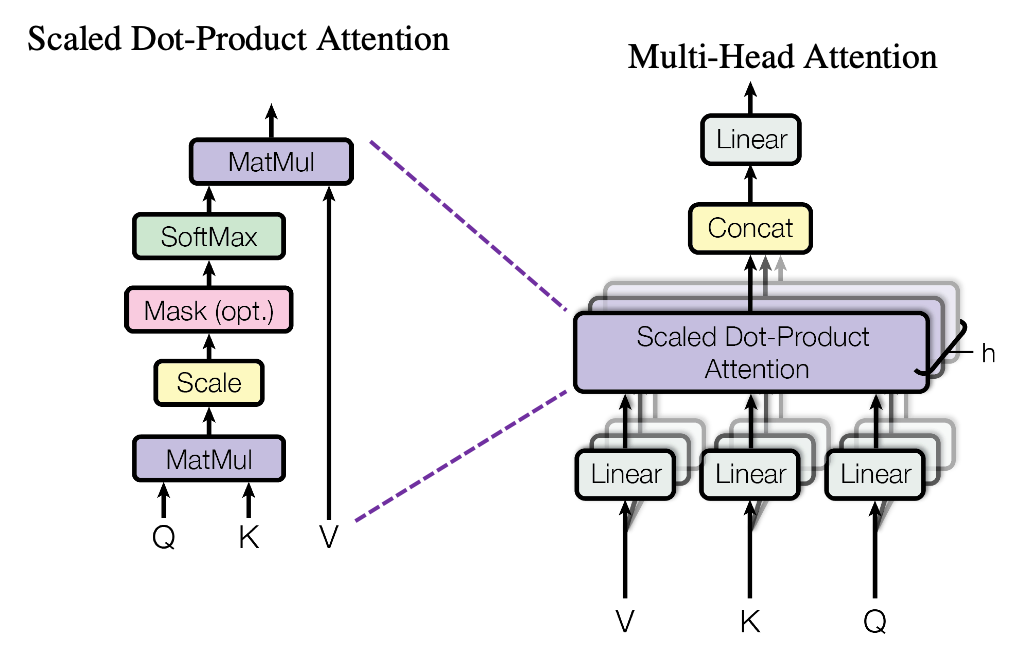
\includegraphics[width=0.5\textwidth]{img/1-section/Attention.png} 

The dominant approach is to pre-train on a \textbf{huge amount of samples and then fine-tune on a smaller task-specific datasets}.

\end{frame}

\begin{frame}
\frametitle{What about computer vision?}
In computer vision before, \textbf{convolutional architectures were dominant} before ViT.

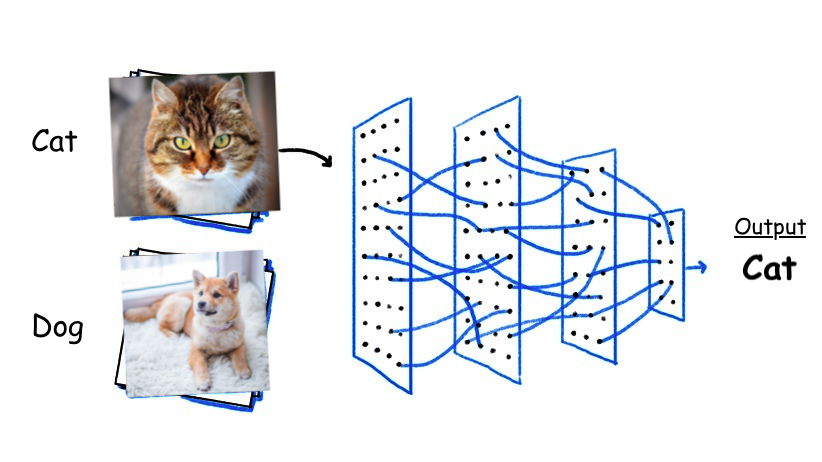
\includegraphics[width=0.5\textwidth]{img/1-section/classification.png} 

\begin{itemize}
    \item Multiple works try combining \textbf{CNN-like architectures with self-attention}
    \item Needed scalability with modern HW.
\end{itemize}

\end{frame}

\begin{frame}
\frametitle{Transformer architectures directly to images}
With Vision transformer the end goal is to \textbf{apply a standard Transformer architectures directly to images}, with the fewest possible modifications
\begin{center}
    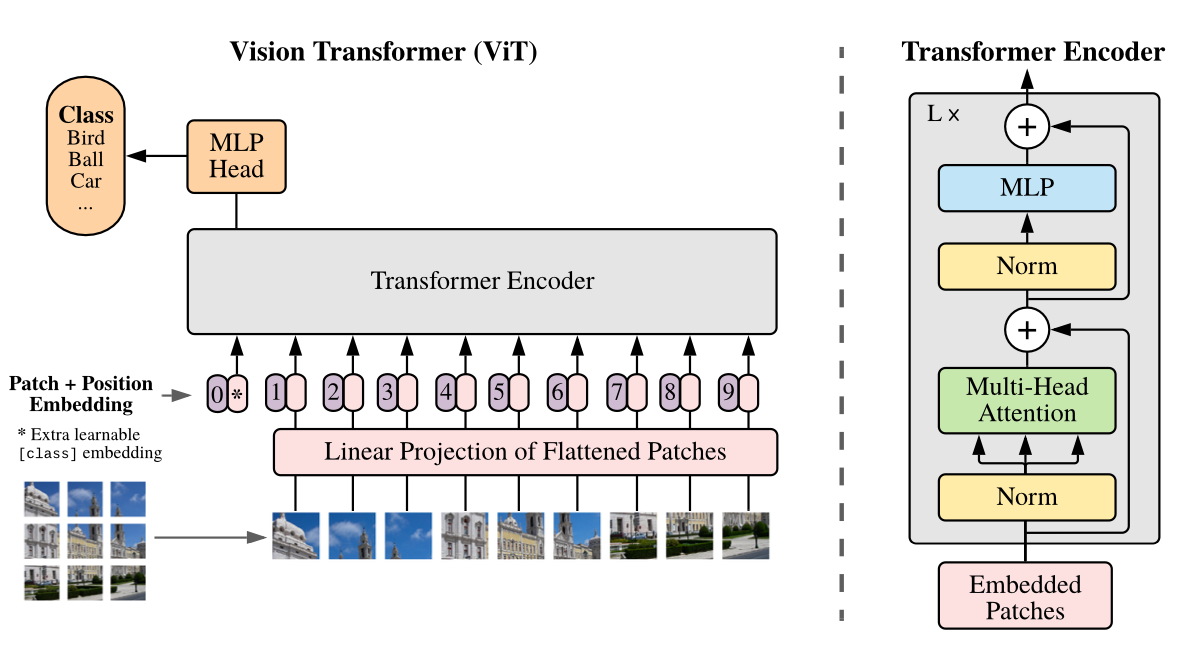
\includegraphics[width=0.8\textwidth]{img/1-section/Vision transformer.png} 
\end{center}

\end{frame}